\begin{frame}
\frametitle{}
Thomas Simpson (1710 - 1761), an English mathematician developed a method for approximating the area under the curve by second-degree polynomials. \\
\begin{center}
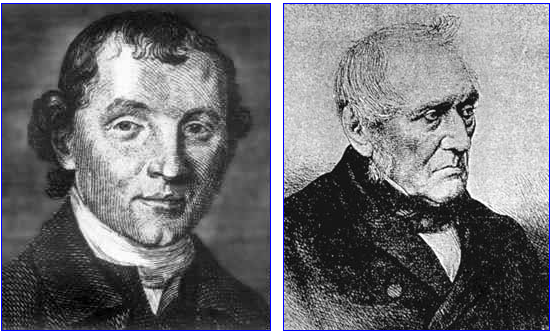
\includegraphics[width=.7\linewidth]{../../modules/approximate-integration/pictures/Simpson}
\end{center}
%Thomas Simpson was born in Leicestershire on August 20, 1710, and died on May 14, 1761. His father was a weaver and he owed his education to his own efforts. His mathematical interests were first aroused by the solar eclipse which took place in 1724, and with the aid of a fortune-telling pedlar he mastered Cocker's Arithmetic and the elements of algebra. He then gave up his weaving and became an usher at a school, and by constant and laborious efforts improved his mathematical education, so that by 1735 he was able to solve several questions which had been recently proposed and which involved the infinitesimal calculus. He next moved to London, and in 1743 was appointed professor of mathematics at Woolwich, a post which he continued to occupy till his death. 
%The works published by Simpson prove him to have been a man of extraordinary natural genius and extreme industry. The most important of them are his Fluxions, 1737 and 1750, with numerous applications to physics and astronomy; his Laws of Chance and his Essays, 1740; his theory of Annuities and Reversions (a branch of mathematics that is due to James Dodson, died in 1757, who was a master at Christ's Hospital, London), with tables of the value of lives, 1742; his Dissertations, 1743, in which the figure of the earth, the force of attraction at the surface of a nearly spherical body, the theory of the tides, and the law of astronomical refraction are discussed; his Algebra, 1745; his Geometry, 1747; his Trigonometry, 1748, in which he introduced the current abbreviations for the trigonometrical functions; his Select Exercises, 1752, containing the solutions of numerous problems and a theory of gunnery; and lastly, his Miscellaneous Tracts, 1754. 
%The work last mentioned consists of eight memoirs, and these contain his best known investigations. The first three papers are on various problems in astronomy; the fourth is on the theory of mean observations; the fifth and sixth on problems in fluxions and algebra; the seventh contains a general solution of the isoperimetrical problem; the eighth contains a discussion of the third and ninth sections of the Principia, and their application to the lunar orbit. In this last memoir Simpson obtained a differential equation for the motion of the apse of the lunar orbit similar to that arrived at by Clairaut, but instead of solving it by successive approximations, he deduced a general solution by indeterminate coefficients. The result agrees with that given by Clairaut. Simpson solved this problem in 1747, two years later than the publication of Clairaut's memoir, but the solution was discovered independently of Clairaut's researches, of which Simpson first heard in 1748. 

%Facts about Cocker's Arithmetic, as discussed in Edward Cocker (English mathematician):
%reputed English author of Cocker’s Arithmetic, a famous textbook, the popularity of which gave rise to the phrase “according to Cocker,” meaning “quite correct.”



\end{frame}
% % % % % % % % % % % % % % % % % % % % % % % % % % % % % % % %
% % % % % % % % % % % % % % % % % % % % % % % % % % % % % % % %
%\begin{frame}
%\frametitle{}
%\tiny Thomas Simpson was born in Leicestershire on August 20, 1710, and died on May 14, 1761. His father was a weaver and he owed his education to his own efforts. His mathematical interests were first aroused by the solar eclipse which took place in 1724, and with the aid of a fortune-telling pedlar he mastered Cocker's Arithmetic and the elements of algebra. He then gave up his weaving and became an usher at a school, and by constant and laborious efforts improved his mathematical education, so that by 1735 he was able to solve several questions which had been recently proposed and which involved the infinitesimal calculus. He next moved to London, and in 1743 was appointed professor of mathematics at Woolwich, a post which he continued to occupy till his death. 
%The works published by Simpson prove him to have been a man of extraordinary natural genius and extreme industry. The most important of them are his Fluxions, 1737 and 1750, with numerous applications to physics and astronomy; his Laws of Chance and his Essays, 1740; his theory of Annuities and Reversions (a branch of mathematics that is due to James Dodson, died in 1757, who was a master at Christ's Hospital, London), with tables of the value of lives, 1742; his Dissertations, 1743, in which the figure of the earth, the force of attraction at the surface of a nearly spherical body, the theory of the tides, and the law of astronomical refraction are discussed; his Algebra, 1745; his Geometry, 1747; his Trigonometry, 1748, in which he introduced the current abbreviations for the trigonometrical functions; his Select Exercises, 1752, containing the solutions of numerous problems and a theory of gunnery; and lastly, his Miscellaneous Tracts, 1754. 
%The work last mentioned consists of eight memoirs, and these contain his best known investigations. The first three papers are on various problems in astronomy; the fourth is on the theory of mean observations; the fifth and sixth on problems in fluxions and algebra; the seventh contains a general solution of the isoperimetrical problem; the eighth contains a discussion of the third and ninth sections of the Principia, and their application to the lunar orbit. In this last memoir Simpson obtained a differential equation for the motion of the apse of the lunar orbit similar to that arrived at by Clairaut, but instead of solving it by successive approximations, he deduced a general solution by indeterminate coefficients. The result agrees with that given by Clairaut. Simpson solved this problem in 1747, two years later than the publication of Clairaut's memoir, but the solution was discovered independently of Clairaut's researches, of which Simpson first heard in 1748. 

%Facts about Cocker's Arithmetic, as discussed in Edward Cocker (English mathematician):
%reputed English author of Cocker's Arithmetic, a famous textbook, the popularity of which gave rise to the phrase ``according to Cocker", meaning ``quite correct".



%\end{frame}
% % % % % % % % % % % % % % % % % % % % % % % % % % % % % % % %
% % % % % % % % % % % % % % % % % % % % % % % % % % % % % % % %
\begin{frame}
\begin{theorem}
If $P(x)=Ax^2 + Bx + C$, then
\[
\int P(x)\; dx = \frac{b-a}{6}\left(P(a)+4P\left(\frac{a+b}{2}\right)+P(b) \right)
\]
\end{theorem}

\only<2>{
\movie[autostart]{}{../../modules/approximate-integration/doh.au}
\begin{center}
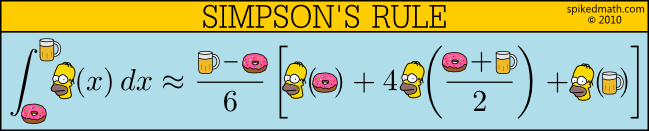
\includegraphics[width=.7\linewidth]{../../modules/approximate-integration/pictures/Simpson2}
\end{center}
}
\end{frame}
% % % % % % % % % % % % % % % % % % % % % % % % % % % % % % % %
% % % % % % % % % % % % % % % % % % % % % % % % % % % % % % % %
\begin{frame}
\frametitle{Simpson's Rule}


We divide the interval into $ n $ subintervals, $ n $ MUST be even.
Instead of straight lines we draw parabolas through  each group of three consecutive points. This approximates the original curve for finding definite integral.\\

\begin{columns}

  \begin{column}{.5\textwidth}
\begin{tikzpicture}[scale=.5]
\coordinate (p1) at (0.7,3);
\coordinate (p2) at (1,3.3);
\coordinate (p3) at (2,2.5);
\coordinate (p4) at (3,2.5);
\coordinate (p5) at (4,3.5);
\coordinate (p6) at (5,4.1);
\coordinate (p7) at (6,3.4);
\coordinate (p8) at (7,4.1);
\coordinate (p9) at (8,4.6);
\coordinate (p10) at (9,4);
\coordinate (p11) at (9.5,4.7);

% The cyan background
%\fill[cyan!10] 
%  (p2|-0,0) -- (p2) -- (p3) -- (p4) -- (p5) -- (p6) -- (p7) -- (p8) -- (p9) -- (p10) -- (p10|-0,0) -- cycle;
% the dark cyan stripe
\only<2-3>{ \fill[yellow,draw=black]  
(p2|-0,0) to (p2) [out=0,in=150] to (p3) [out=-50,in=230] to  (p4) [out=-90,in=90] to (p4|-0,0);
} %
\only<4->{ \fill[yellow,draw=black]  
(p4|-0,0) to (p4) [out=30,in=220] to (p5) [out=50,in=150] to  (p6) [out=-90,in=90] to (p6|-0,0);
} %
% the curve
\draw[thick,cyan] 
    %(p1) to[out=70,in=180] 
    (p2) to[out=0,in=150] 
    (p3) to[out=-50,in=230] (p4) to[out=30,in=220] 
    (p5) to[out=50,in=150] (p6) to[out=-30,in=180] 
    (p7) to[out=0,in=230] (p8) to[out=40,in=180] 
    (p9) to[out=-30,in=180] (p10); 
    % to[out=0,in=260] (p11);
% Simpson parabola
\only<2-3>{\draw[thick,red] 
    %(p1) to[out=70,in=180] 
    (p2) to[out=0,in=150] 
    (p3) to[out=-50,in=230] 
    (p4) ; 
    } %
\only<4->{\draw[thick,red] 
    (p4) to[out=30,in=220] 
    (p5) to[out=50,in=150] 
    (p6) ; 
    } %
\only<2-3>{    
\node[above,font=\footnotesize] at (1.5,0) {$\Delta x$};
\node[above,font=\footnotesize] at (2.5,0) {$\Delta x$};
\node[above] at (2,1) {$A_1$};
} %
\only<4->{
\node[above,font=\footnotesize] at (3.5,0) {$\Delta x$};
\node[above,font=\footnotesize] at (4.5,0) {$\Delta x$};
\node[above] at (4,1) {$A_2$};
} %        
% vertical lines and labels
\foreach \n/\texto in {2/{a},3/{x_1},4/{x_2},5/{x_3},6/{x_4},7/{},8/{},9/{x_{n-1}},10/{b}}
{
  \draw (p\n|-0,0) -- (p\n);
  \node[below,text height=1.5ex,text depth=1ex,font=\small] at (p\n|-0,0) {$\texto$};
}
% The axes
\draw[->] (-0.5,0) -- (10,0) coordinate (x axis);
\draw[->] (0,-0.5) -- (0,6) coordinate (y axis);
% labels for the axes
\node[below] at (x axis) {$x$};
\node[left] at (y axis) {$y$};
% label for the function
\node[above,text=cyan] at (p11) {$y=f(x)$};
\end{tikzpicture}
\end{column}

\begin{column}{.5\textwidth}
\uncover<3->{%
%$\ds  \Delta x=\frac{b-a}{n} $
\begin{align*}
A_1 & =\frac{2\Delta x}{6}\left(f(x_0)+4f(x_1)+f(x_2)\right)\\
& =\frac{\Delta x}{3}\left(f(x_0)+4f(x_1)+f(x_2)\right)  
\end{align*}
}
\uncover<4->{%
$ \ds A_2= \frac{\Delta x}{3}\left(f(x_2)+4f(x_3)+f(x_4)\right) $
} %
\end{column}


\end{columns}


%\hspace*{2cm}



%\only<1>{
%\includegraphics[width=.5\linewidth]{../../modules/approximate-integration/pictures/S1}
%}
%\uncover<2->{%
%\includegraphics[width=.5\linewidth]{../../modules/approximate-integration/pictures/S2}
%}

\uncover<5->{%
The sum of the areas $ A_1+A_2+\cdots+A_{\frac{n}{2}} $ is denoted $ S_n $:
\scriptsize{
\begin{align*}
S_n & =\frac{\Delta x}{3}\left[ \left( f(x_0)+4f(x_1)+f(x_2)\right)+ \left(f(x_2)+4f(x_3)+f(x_4)\right)+ \cdots + \left(f(x_{n-2})+4f(x_{n-1})+f(x_n)\right) \right]\\
& =\frac{\Delta x}{3}\left[  f(x_0)+4f(x_1)+2 f(x_2)  + 4f(x_3)+ 2f(x_4) + \cdots + 2f(x_{n-2})+4f(x_{n-1})+f(x_n) \right]  
\end{align*}
}
}

\end{frame}
% % % % % % % % % % % % % % % % % % % % % % % % % % % % % % % %
% % % % % % % % % % % % % % % % % % % % % % % % % % % % % % % %
\begin{frame}
\frametitle{}
\begin{theorem}[Simpson's Rule]
For $ n $ even, Simpson's Rule states that $ \ds \int_a^b f(x)\; dx \approx S_n $, where
\[ S_n= \frac{\Delta x}3\left[f(x_0)
+4f(x_1)+2f(x_2)+4f(x_3)+\dots +4f(x_{n-1})+f(x_n)\right].
\]
Here, $n$ must be even.  The pattern of coefficients is $1, 4, 2, 4, 2, 
\dots, 4, 2, 4, 1$.  As it happens,
\[S_{2n}=\frac 1 3 T_n + \frac 2 3 M_n.\]
\end{theorem}
\end{frame}
% % % % % % % % % % % % % % % % % % % % % % % % % % % % % % % %

